\documentclass{article}

\usepackage{amsmath,amssymb,amsfonts,amsthm}
\usepackage{graphicx,psfrag,wasysym,multirow}
\usepackage[pdftex,bookmarks=true]{hyperref}
\usepackage{caption,subcaption}
\usepackage[usenames,dvipsnames]{xcolor}
\usepackage{authblk,hyperref,xcolor}
\usepackage[english]{babel}
\usepackage{natbib}
\usepackage{marg}
%\usepackage{showlabelsjr}
\bibliographystyle{abbrvnat}
\setcitestyle{authoryear,open={(},close={)}}
\newtheorem{thm}{Theorem}

\DeclareMathOperator{\Tr}{Tr}
\DeclareMathOperator*{\argmin}{arg\,min}
\DeclareMathOperator*{\argmax}{arg\,max}
%%%%%%%%%%%%%%%%%%%%%%%%%%%%%%%%%%%%%%%%%%%%


\author[1]{Jonathan Sidi}
\author[1]{Ya'acov Ritov}
\author[2]{Lyle Ungar}

\affil[1]{Department of Statistics, Hebrew University in Jerusalem}
\affil[2]{Computer and Information Statistics, University of Pennsylvania}

\renewcommand\Authands{ and }
\title{Regularization and Classification of Linear Mixed Models via the Elastic Net Penalty \\ with Application to the Good Judgment Project\footnote{This research was supported by a research contract to the University of Pennsylvania and the University of California from the Intelligence Advanced Research Projects Activity (IARPA) via the Department of Interior National Business Center contract number D11PC20061. The U.S. Government is authorized to reproduce and distribute reprints for Government purposes notwithstanding any copyright annotation thereon. Disclaimer: The views and conclusions expressed herein are those of the authors and should not be interpreted as necessarily representing the official policies or endorsements, either expressed or implied, of IARPA, DoI/NBC, or the U.S. Government.}}

\usepackage{Sweave}
\begin{document}
\Sconcordance{concordance:lmmen_paper.tex:lmmen_paper.Rnw:%
1 30 1 1 0 2 1 1 87 221 1 2 2 7 1 2 2 16 1 1 7 1 2 19 1}




\clearpage
\maketitle
\thispagestyle{empty}

 \vspace{1cm}
 \begin{center}
  Corresponding Author: Jonathan Sidi, Email: \href{mailto:yoni.sidi@mail.huji.ac.il}{yoni.sidi@mail.huji.ac.il}
 \end{center}
 
  \vspace{1cm}
  \textbf{Keywords}: Linear mixed model; Elastic Net penalty; Variable selection; Probabilistic forecast



\newpage
\begin{abstract}
Advances in the field of model selection and prediction via regularization has forged the ability of a variety of disciplines to classify and model large-scale data. Widely used methods which apply penalties in classification are the Least Absolute Shrinkage and Selection Operator (LASSO), the Adaptive LASSO and the Elastic Net. These methods have predominately been used to classify problems of Generalized Linear Models (GLM) in which the dependency of the covariance structure is assumed to be independent. This assumption is not commonly met in practical data and the ability to model such dependencies is integral in fitting the data correctly, such data is modeled using Linear Mixed Models (LMM). Recent research applying LASSO and Adaptive LASSO to LMM's has produced promising initial results of identifying both the random and fixed effects found in data, proving both consistency and an oracle optimality. However, an inherent drawback to those variable selection methods is their performance under high correlation between covariates. To overcome this we introduce the Elastic Net penalty to LMM selection. This penalty has been found to reduce the prediction error in data with high correlation between variables; such a characteristic can be utilized in more complex data designs while optimizing the LMM problem. Findings are tested through simulations and a case study using data accumulated in an longitudinal study where probabilistic forecasts are derived from crowd sentiment. The data structure consists of repeated measures and a large number of fixed and random covariates.
\end{abstract}
\newpage
	\section{Introduction}
		Generalized Linear Mixed models (GLMM) \cite{BreslowClayton1993} have been applied in a variety of fields to study data designs with between-subject variation. Such designs include longitudinal, repeated measures and clustered data and have been studied thoroughly in the low dimension setting, e.g., \cite{Bates2010} and \cite{searle1992variance}. In these settings the linear predictor contains in addition to fixed effects, found in Generalized Linear Models (GLM), latent random effects which capture the unique design pertaining to the data. These random effects usually are assumed to have a centered parametric distribution belonging to the exponential family.
		
  Advances in the field of model selection and prediction via regularization, using different penalty terms, has forged the ability of a variety of disciplines to classify and model large-scale data. Widely used methods which apply penalties in classification are the Least Absolute Shrinkage and Selection Operator (LASSO), the Adaptive LASSO and the Elastic Net. These methods have predominately been used to classify problems of GLM, \cite{FHT2010} and \cite{VandeGeer2008}, in which the dependency of the covariance structure is assumed to be independent. This assumption in practical data is not commonly met and the ability to model such dependencies is integral in fitting the data correctly, such data is modeled using Linear Mixed Models (LMM) and GLMMs.

  Recent research \cite{SchelldorferBuhlmann2011},\cite{fan2012variable} and \cite{BKG2010} apply the LASSO, SCAD and Adaptive LASSO respectively to LMMs and have produced promising initial results of identifying both the random and fixed effects found in data, proving both consistency and an oracle optimality. These articles apply a penalty to the LMM optimization, while achieving this each in a distinct approach. This paper, proposes a new algorithm, LMMEN that attempts to utilize the advantages of each method and submit a new type of penalty which better captures the design of the LMM. %Comparisons to each method will be done through simulations and a case study.
		
\begin{subsection}{Model} \label{jrange}
    The GLMM is defined as having $m$ subjects in the sample. For the $i$th subject the response variable is denoted as $y_{ij}$ for the $j$th observation, where $j=1 \dots n_i$ and let $N=\sum_{i=1}^{m}n_i$. The training data \textbf{X} can be defined as two groups of covariates: the fixed effects covariates vector denoted as $x_{ij}$ with dimensions $p\times 1$ and the random effects covariates vector denoted as $z_{ij}$ with dimensions $q\times 1$.

    $y_{ij}$ are assumed to be conditionally independent given the subject-specific random effects, $b_i$, with a conditional mean $E[y_{ij}|b_i]=\mu_{ij}$ and a conditional variance $var(y_{ij}|b_i)=\phi\omega^{-1}_{ij}\nu(\mu_{ij})$. Where $\phi$ is a positive dispersion parameter, $\omega_{ij}$ is a pre-specified weight, and $\nu(\cdot)$ is the variance function. The relationship between $\mu_{ij}$ to \textbf{X} is defined as
%		
		\begin{equation*}
		g(\mu_{ij})=x'_{ij}\beta+z'_{ij}b_i,
		\end{equation*}
%		
		where $g(\cdot)$ is a strictly increasing link function, $\beta$ is the fixed effects coefficient vector for $x$ and $b_i$ is the subject-specific random effects for $z$. $y_{ij}$ are assumed to be independent and of the form $y_{ij}|b_i\sim F_y$ and $b_i$ is assumed to be of the form $b_i\sim F_b$. The distributions  $F_y$ and $F_b$ are predominately assumed to be normal, i.e.:
%
		\begin{eqnarray*}
				F_y&\sim& N(\mu_{ij},\phi\omega^{-1}_{ij}\nu(\mu_{ij}))\\
				F_b&\sim& N(0,D(\psi)),
		\end{eqnarray*}
%
where $\psi$ is a $c \times 1$ vector of variance components in the covariance matrix of the random effects $D$. Under the identity link function with normal distribution we define the LMM
%
		\begin{equation}
		\label{eq:LMM}
		\begin{split}
		y_i&=x'_{ij}\beta+z'_{ij}b_i+\epsilon_i,\\
		\epsilon_i&\sim N(0,\sigma^2I_{n_i}).
		\end{split}
		\end{equation}
%		
\cite{McCullochNeuhaus2011} state that distribution specification may be affected by basic characteristics of the random effects distribution, such as dependence on a covariate or the cluster sample size.
For example, the mean or variance of $F_b$ depends on a covariate. When the mean of the random effects distribution depends on a covariate, a fundamental relationship is
introduced between the covariate and the distribution, potentially creating a serious bias in estimating the form of the relationship between the covariate and the outcome. \cite{heagerty2001misspecified} show that the impact of highly unequal variances can lead to substantial bias. Such bias from distribution specification can cause unintended inference when testing between and within cluster covariates.
\end{subsection}

\cite{SchelldorferBuhlmann2011} defined the GLMMLASSO, which solves the log likelihood of the LMM problem via integral approximation (Laplace approximation) and submit the approximated function to numerical optimization. The advantage of integral approximation methods is to provide an actual objective function for optimization, which enables one to perform likelihood ratio tests among nested models and to compute likelihood-based fit statistics. The disadvantage of these methods is the difficulty of accommodating crossed random effects and multiple subject effects, and the inability to accommodate residual effect covariance structures, or even only residual effect over-dispersion. Moreover, the number of random effects should be small for integral approximation methods to be practically feasible. This disadvantage could potentially inhibit the estimation of random effects in a high dimensional data setting. The penalty term which is used on the approximated likelihood function is the $L_1$ penalty. The algorithm proposed penalizes only the fixed effects in the model, thereby estimating the parameters $\lbrace\beta,\theta,\phi\rbrace$ and predicting the random effects vector $b$ using those estimates. The size of the tuning parameter is calculated  in two steps: first via the AIC criterion to generate a relevant set of variables and secondly via the BIC criterion to select the final set of active fixed effects which is an unbiased estimator of degrees of freedom in linear models.

\cite{fan2012variable} introduce a class of variable selection methods for the fixed effects using a penalized profile likelihood, provided that the random effects vector has a nonsingular covariance matrix. This penalized profile likelihood is equivalent to the penalized quadratic loss function of fixed effects readily found in penalized least squared methods, such as LARS \cite{efron2004least}. Random effects are selected under the constraint that the dimension of the fixed effects is smaller than the sample size. They describe an iterative solution for high dimensionality of both the fixed and random effect by which of selecting the fixed effects using the penalized least squares by ignoring all random effects to reduce the number of fixed effects to below sample size. Then in the second step, with the selected fixed effects, they select random effects and finally using the selected random effects refine the fixed effects selections.

\cite{BKG2010} apply linearization (Taylor expansion) to solve the LMM which is more aptly suited in models with correlated errors, a large number of random effects, crossed random effects, and multiple types of subjects. The disadvantages of this approach include the absence of a true objective function for the overall optimization process and potentially biased estimates. The likelihood function is reparameterized via a modified Cholesky decomposition of the random effects covariance structure \cite{ChenDunson2003}. This augmentation allows for penalties on both the fixed and random effects. The penalty used in the optimization is the Adaptive Lasso, \cite{Zou2006}, which allows for large amount of shrinkage applied to the zero-coefficients while smaller amounts are used for the non-zero ones which then results in an estimator with improved efficiency and selection properties. The level of the tuning parameter is calculated using the BIC criterion.

\section{Reparameterization of the Generalized Linear Mixed Model}
This paper will utilize the reparameterization of the LMM model initially defined in \cite{ChenDunson2003}, and used in \cite{BKG2010}. The reparameterization offers a simple design which regularization penalties can be easily applied to the fixed and random effects simultaneously. The covariance matrix of the random effects $D$ is factorized as follows:
%
		\begin{equation}
			\label{eq:fact}
			D=\Lambda\Gamma\Gamma'\Lambda,
		\end{equation}
%		
where $\Lambda=\mathop{\rm diag}(d_1,\dots,d_q)$ is a $q\times q$ non-negative diagonal matrix with elements proportional to standard deviations  of the random effects, and $\Gamma$ is a lower triangular matrix that relates to the correlations among the random effects with the $(l,m)$ elements denoted $\gamma_{lm}$. The elements of $\Lambda$ are defined as possibly equal zero, thus enabling a subset of random effects to be selected. $\Lambda$ and $\Gamma$ are identifiable due to the assumption that:
%
$$d_l\ge 0,\;\gamma_{ll}=1 \text{, and }\gamma_{lr}=0 \text{, for } l=1,\dots,q;\:r=l+1,\dots,q.$$
%		
Applying the modified decomposition \eqref{eq:fact} to the LMM model \eqref{eq:LMM} the reparameterized LMM is defined, where the covariance matrix of \textbf{$b_i$} is a function of $\Lambda,\Gamma$:
%		
		\begin{equation*}
			y_i=x'_i\beta+z'_i\Lambda\Gamma b_i+\epsilon_i.
		\end{equation*}
%
	\section{Simultaneous Variable Selection and Estimation via Regularization Penalties}	
The Adaptive LASSO has been used as the penalty function on the modified LMM by \cite{BKG2010} due to its oracle qualities. Although, there are drawbacks to its use, the primary disadvantage is that candidate covariates correlated to variables chosen in the active set are dropped from the final solution. This characteristic has been found to be a drawback in large scale data with grouped covariates. Moreover, when solving the likelihood of the LMM we can see that the fixed and random effects are dependent.
%		
		\begin{equation}
		\label{eq:Loglik}
		L(\phi|y,b)=-\frac{N+mq}{2}\log(\sigma^2)-\frac{1}{2\sigma^2}(||y-Z(I_m\otimes \Lambda)(I_m\otimes \Gamma) b-X\beta||^2+b'b),
		\end{equation}
		with $\otimes$ denoting the Kronker product, $Z$ is a block diagonal matrix of $Z_i$, $I_m$ is the identity matrix of dimension $m$.
%

To overcome these issues we apply a variation on the Elastic Net penalty to the reparameterized likelihood function, \eqref{eq:Loglik}. The standard Elastic Net penalty denoted as $P$, \cite{FHT2010}, is designed to be applied on a fixed effects model where only $\beta$ is penalized, as seen in \eqref{eq:EN} below. In this formulation the problem of collinearity is addressed ($L_2$ penalty) in conjunction with shrinkage of redundant variables  ($L_1$ penalty).
%		
			\begin{equation}
			\begin{split}
			\hat{\beta}&=\argmin\limits_{\beta\in R^{p+1}}\left[\frac{1}{2N}\sum\limits_{i=1}^{N} (y_i-x_i'\beta)^2 + P(\beta)\right]\\
			P(\beta)&=\lambda_2\sum\limits_{j \in P}\beta_j^2+\lambda_1\sum\limits_{j \in P}|\beta_j|.
			\end{split}
			\label{eq:EN}
			\end{equation}
%
We augment \eqref{eq:EN}, while keeping the overall structure and characteristics of the Elastic Net, i.e., the quadratic structure in the $L_2$ penalty. The reparameterization of the LMM allows the penalty function, $\tilde{P}(\beta,d)$, to be dependent on both the fixed and random effects in the model.

In addition, correlated random effects can be included in the final model selection, whereas in the Adaptive LASSO settings this was not possible, thus overcoming the problematic testing of simultaneous random effects, \cite{ChenDunson2003}. The objective function of the LMMEN is defined as the following:
%
\begin{equation}
\label{eq:MLE-EN}
  \begin{split}
    Q(\phi|y,b)&=||y-Z\Lambda\Gamma b-X\beta||^2+\tilde{P}(\beta,d)\\
    \tilde{P}(\beta,d)&=\lambda_2^f\sum\limits_{i\in P}\beta_i^2+\lambda_2^r\sum\limits_{j\in Q}d_j^2+\lambda_1^f\sum\limits_{i \in P}|\beta_i|+\lambda_1^r\sum\limits_{j \in Q}|d_j|.
  \end{split}
\end{equation}
%
Where $\tilde{P}$ and $Q(\phi)$ denote the penalty applied to the likelihood and the penalized log-likelihood. When the final model is not a mixed effects model, but either a fixed effects or random effects model then the original form of $P_\alpha$ is applied.
		
% 		\begin{subequations}
% 			\begin{equation}
% 			\label{eq:FEM}	
% 				\tilde{P}_\alpha(\beta,d)|_{||d||=0}=\frac{1}{2}(1-\alpha)(\lambda_2^f\sum\limits_{i\in P}\beta_i^2)+\alpha(\lambda_1^f\sum\limits_{i \in P}|\beta_i|)
% 			\end{equation}
% 			\begin{equation}
% 			\label{eq:REM}
% 				\tilde{P}_\alpha(\beta,d)|_{||\beta||=0}=\frac{1}{2}(1-\alpha)(\lambda_2^r\sum\limits_{j\in Q}d_j^2)+\alpha(\lambda_1^r\sum\limits_{j \in Q}|d_j|)
% 			\end{equation}
% 		\end{subequations}

\section{Asymptotics}
Assume that the data $\{(X_i,Z_i,y_i); \text{ } i=1...m\}$ is a random sample of $m$ subjects from a linear mixed-effects model with a probability density function $f(y_i|X_i,Z_i,\phi)$. Let $y_i$ be an $n_i \times 1$ response measurements for subject $i$, $X_i$ be an $n_i \times p$ design matrix of explanatory variables, and $Z_i$ be an $n_i \times q$ design matrix of random effects.

Let $\phi=(\beta',d',\gamma')'$ be a vector of size $k \times 1$, where $\beta \in \mathbb{R}^p$, $d \in \mathbb{R}^q$ and $\gamma$ is of the dimension $\frac{q(q-1)}{2}$. $p=m^{\alpha}$ is the number of fixed effects, and $q=m^{\delta}$ the number of the random effects to be estimated. Then number of free elements in the covariance matrix of the random effects, $\Phi$, is $\frac{q(q-1)}{2}$.

In \cite{BKG2010} the hyperparameters satisfy $\alpha < 1$ and $\delta < 1$ giving a setup of $m>p$, $m>q$. The total number of unknown hyper parameters is $k=p+\frac{q(q+1)}{2}\ll m$. In this paper we are letting $\alpha > 1$ , $\delta < 1$ giving a framework of $m<p$ , $m>q$, i.e. a high-dimensional problem. The total number of unknown parameters that are estimated in this framework is $k=m^{\alpha}+\frac{m^{\delta}(m^{\delta}+1)}{2}\gg m$.

Let $L_i(\phi)=\text{log}(f(y_i|X_i,Z_i,\phi))$ denote the contribution of observation $i$ to the log-likelihood function, given by:
\begin{equation}
L_i(\phi)= -\frac{1}{2} \mathop{\rm log}|\textbf{V}_i|-\frac{1}{2}(\textbf{y}_i - \textbf{X}_i\beta)'\textbf{V}_i^{-1}(\textbf{y}_i-\textbf{X}_i\beta),
\label{eq:loglik}
\end{equation}
where $\textbf{V}_i=\sigma^2(Z_i\Lambda\Gamma\Gamma'\Lambda Z_i+I_{n_i})$. Denoting the true value of $\phi$ as $$\phi_0=(\varphi_{10},\dots,\varphi_{k0}) '=( \phi_{10}',\phi_{20}')',$$ where $\phi_{10}=(\beta_{10}',d_{10}',\gamma_{10}')'$ is an $s \times 1$ vector whose components are non-zero and $\phi_{20}$ are the $(k-s)$ remaining components of $\phi_0$ such that $\phi_{20}=0$. Accordingly, let $\phi=( \phi_{1}',\phi_{2}')'$.
To present the theorems the following regularity conditions are imposed:
%
\begin{description}
	\item[C1\label{C1}]
		The Fisher information matrix $I(\phi_{10})$ knowing $\phi_{20}=0$ is finite and positive definite.
	\item[C2\label{C2}]
		There exists an open subset $\Theta$ of $\mathbb{R}^k$, containing the true parameter $\phi_0$ such that $L_i(\phi)$ given in \eqref{eq:loglik} admits all third order derivatives, which are continuous and bounded.
		There exists a finite mean function $M_{jlm}(y_i,X_i,Z_i)$ such that $$\left|\frac{\partial^3}{\partial \beta \partial\varphi_l \partial \varphi_m}L_i(\phi)\right|<M(y_i,X_i,Z_i).$$
\end{description}
We have:
\begin{thm}
  \label{thm1}
    Let $\phi_0=(\phi'_{10},0')'$, and the observations follow the LMM model satisfying conditions \nameref{C1} and \nameref{C2}. If  $w_mm^{-1/2}\to\infty$, $(\lambda_1^f+\lambda_1^r)\sqrt s/mw_m\to 0$, $(\lambda_2^f+\lambda_2^r)/m\to 0$, and $(\lambda_2^f+\lambda_2^r)s/mw_m\to 0$, then there exists a local maximizer $\hat{\phi}=\begin{pmatrix}
    \hat{\phi_1} \\ 0 \end{pmatrix}$ of $Q\begin{Bmatrix}\begin{pmatrix}
    \hat{\phi_1} \\ 0 \end{pmatrix}\end{Bmatrix}$ such that $\hat{\phi_1}$ is $w_m$ consistent for $\phi_{10}$.
  \end{thm}

\begin{thm}
\label{thm2}
Let the observations follow the LMM model satisfying conditions \nameref{C1} and \nameref{C2}. If $\lambda_m \rightarrow \infty$ then with probability tending to 1 for any given $\phi_1$ satisfying $||\phi_1-\phi_{10}||_1\le Mm^{-1/2}$ and some constant $M>0$,

  $$ Q\left\lbrace\left(
		\begin{array}{c}
			\phi_1 \\ 0
		\end{array}
		\right)  \right\rbrace
		=\max\limits_{||\phi_2||_1\le Mm^{-1/2}}
	Q\left\lbrace\left(
		\begin{array}{c}
		\phi_1 \\ \phi_2
		\end{array}
		\right)\right\rbrace.
	$$
\end{thm}

\section{Simulations}
Simulation testing the model selection performance were carried out on five scenarios. In each scenario 100 data sets were simulated from a multivariate normal density. $$y_i\sim N(X_i\beta,\sigma^2(Z_i\Psi Z'_i+I_{n_i}))$$
The true values of $(\beta_1,\beta_2)=(1,1)$, and the true variance covariance matrix
		$$ \Psi= \left(
		\begin{array}{ccc}
			9   & 4.8 & 0.6 \\
			4.8 & 4   & 1   \\
			0.6 & 1   & 1
		\end{array}
		\right) $$
The parameterization of the five scenarios are defined in Table \ref{tab:Scenario}.
\begin{table}[h]
		  \centering
\ %vspace{-10pt}
\scalebox{0.8}{
\begin{tabular}{|c|c|c|c|c|c|}
\hline
\multirow{2}{*}{Scenario} &   Subjects & Obs per subject & Fixed Effects & Random Effects & Correlation \\
\cline{2-6}
\multicolumn{ 1}{|c|}{} &          m &      $n_i$ &          p &          q &     $\rho$ \\ \hline
         1 & 30 & 5  & 9 & 4  &  no  \\
         2 & 60 & 10 & 9 & 4  &  no  \\
         3 & 60 & 5  & 9 & 10 &  no  \\
         4 & 60 & 10 & 9 & 4  &  Multicollin \\
         5 & 30 & 5 & 200 & 4  &  p>n \\
         \hline
\end{tabular}}
\caption{Simulation Scenarios}
\label{tab:Scenario}
\end{table}

The first three scenarios are taken from the \cite{BKG2010} to test the LMMEN to its counterpart ``Penalized Linear Mixed Effects Model"  (Pen.LME). The true model under consideration in scenarios 1 and 2 is defined as model \eqref{eq:scen1} and scenario 3 where $X=Z$ as model \eqref{eq:scen2}.
\begin{subequations}
\begin{align}
y_{ij}&=b_{i1}+\beta_1x_{ij1}+\beta_2x_{ij2}+b_{i2}Z_{ij1}+b_{i3}Z_{ij2}+\epsilon_{ij} &\qquad \epsilon_{ij}\sim N(0,1)
\label{eq:scen1}
\\
y_{ij}&=b_{i1}+(\beta_1+b_{i2})x_{ij1}+b_{i3}X_{ij3}+\epsilon_{ij} &\qquad  \epsilon_{ij}\sim N(0,1)
\label{eq:scen2}
\end{align}
\end{subequations}
Scenario 4 tests the model performance under settings that there is a high correlation between fixed variables. The scenario uses the same data as scenario 2 and replaces $X_3$ with a linear combination of {$X_1$,$X_2$} where $X_3=wX_1+(1-w)X_2+\epsilon$ where $\epsilon\sim N(0,\tau)$. This introduces high correlation in the first three fixed effects, in this setting the LASSO and Adaptive Lasso discard one of these fixed effects thus rendering the model selection inferior. The final scenario tests the performance in high dimension settings. The number of fixed effects is increased to 200 and the first 20 are real parameters while the remainder 180 are nuisance, the random effects remain as in the previous scenarios. This scenario can only be run under LMMEN since the initial values are not calculated using the solution of an unpenalized mixed model, as in the Pen.LME.

Figure \ref{fig:glmmensim} depicts the distribution of each parameter estimated within each scenario, where the fixed effects are on the left hand side and the standard deviations of the random effects are on the right hand side. The results of the LMMEN (black) is compared to the Pen.LME (grey). The first three scenarios' results are comparable between the two methods, where the real parameters are chosen consistently. In the fourth scenario the LMMEN selects all the covariates while distributing relatively equal weights to each one. The Pen.LME's adaptive lasso penalty can not discern between the highly correlated variables and sets the 3rd fixed effect near to zero a high percent of the time. In addition, we see that there is no loss of performance in the LMMEN in that it excludes the nuisance fixed effects and correctly estimating the random effects. In the fifth scenario the LMMEN selects the first 20 fixed parameters persistently while setting to zero the nuisance fixed effects, while correctly estimating the random effects.
%
\begin{figure}[t]
\centering
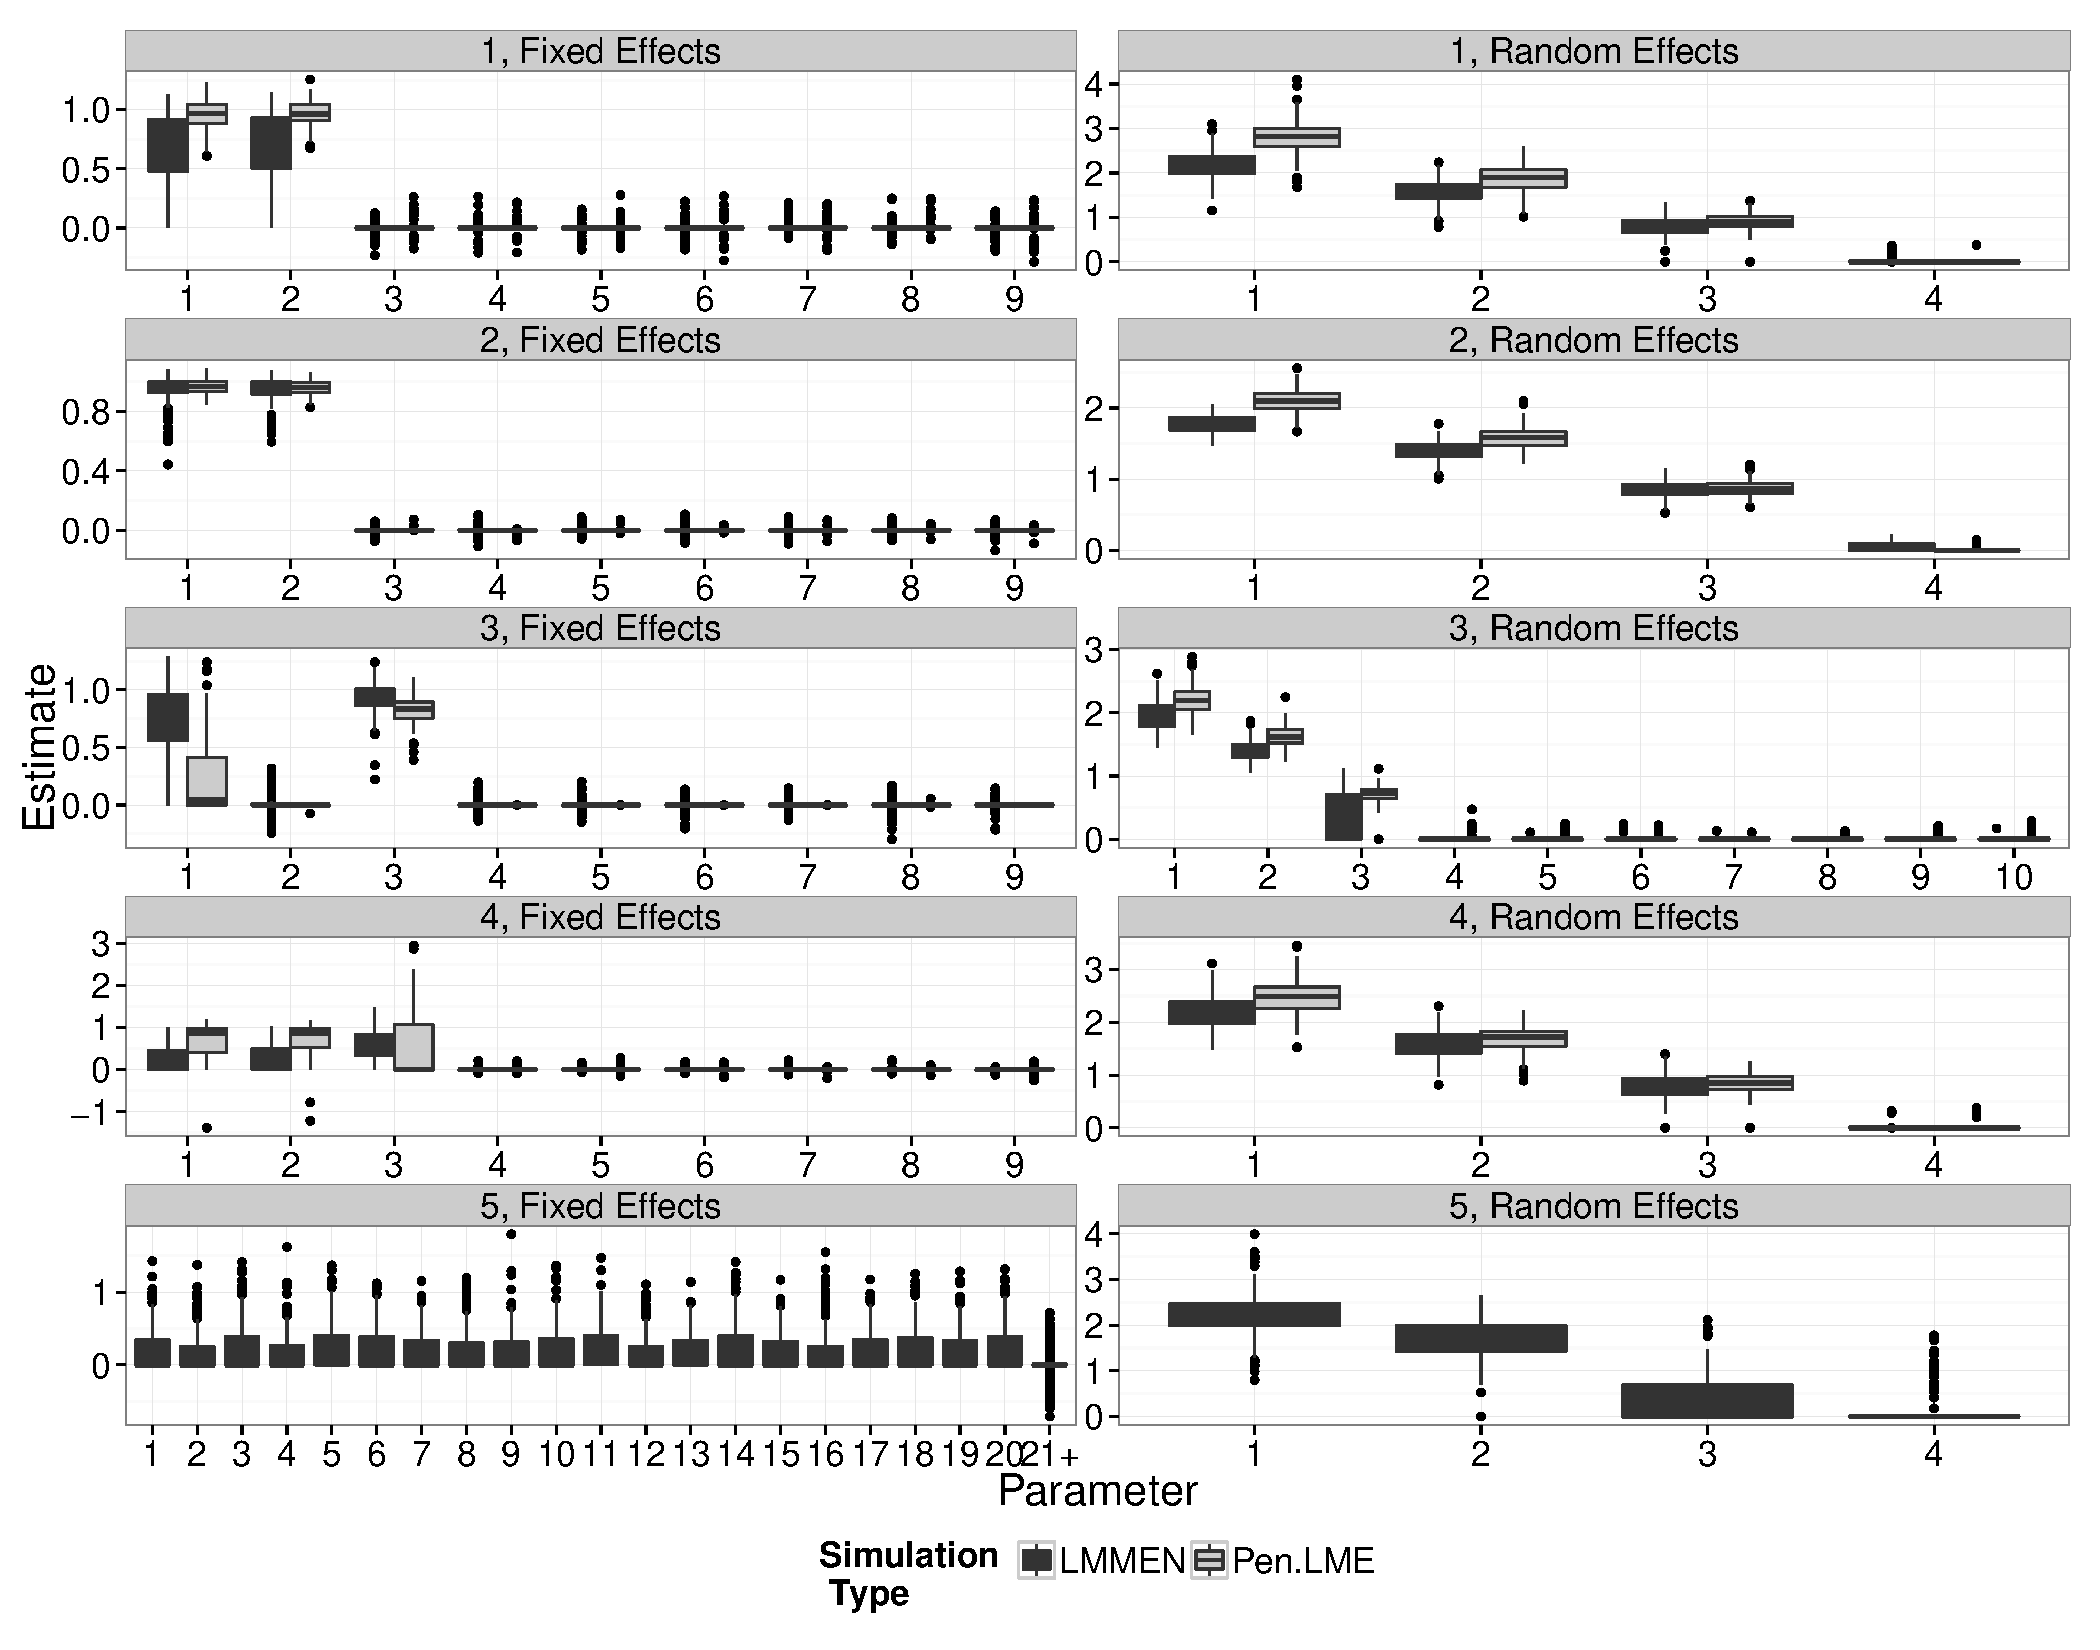
\includegraphics{figs/lmmen_paper-scenario}
\caption{Simulation results of the five scenarios defined in Table \ref{tab:Scenario}. Each row is a different scenario, while the left hand side of the panel depict the distribution of the simulated estimated fixed effects parameters, the right hand side depicts the distribution of the estimated random effect parameters. The grey boxplots are the results of the Pen.LME and the black boxplots are the LMMEN.}
\label{fig:glmmensim}
\end{figure}
%

Figure \ref{fig:oracle} shows the mean percent of variables correctly selected for the whole model, only the fixed effects and only the random effects for each scenario. This measures performance of model selection without the constraint of an oracle property. For example, in the first scenario of LMMEN 89\% of the percent of the variables were correctly selected. We see that the two methods perform similarly, where in the second scenario the Pen.LME out-performed the LMMEN. In high dimension scenario the LMMEN selected 94\% of the correct variables on average. Comparing the performance of selecting the all the parameters perfectly, oracle quality, we see that both selections methods results are tempered. In scenario one, the LMMEN selects the perfect model 38\% of the time, while comparatively the Pen.LME perfectly selects 50\% of the simulations. We see that in the multicollinearity scenario (4), the LMMEN out-performs the Pen.LME selecting all three correct fixed effects 25\% of the time, while the Pen.LME 4\%. As expected the in the fifth scenario the LMMEN was not able to select all 200 variables correctly in any of the simulations.
%
\begin{figure}[h]
\centering
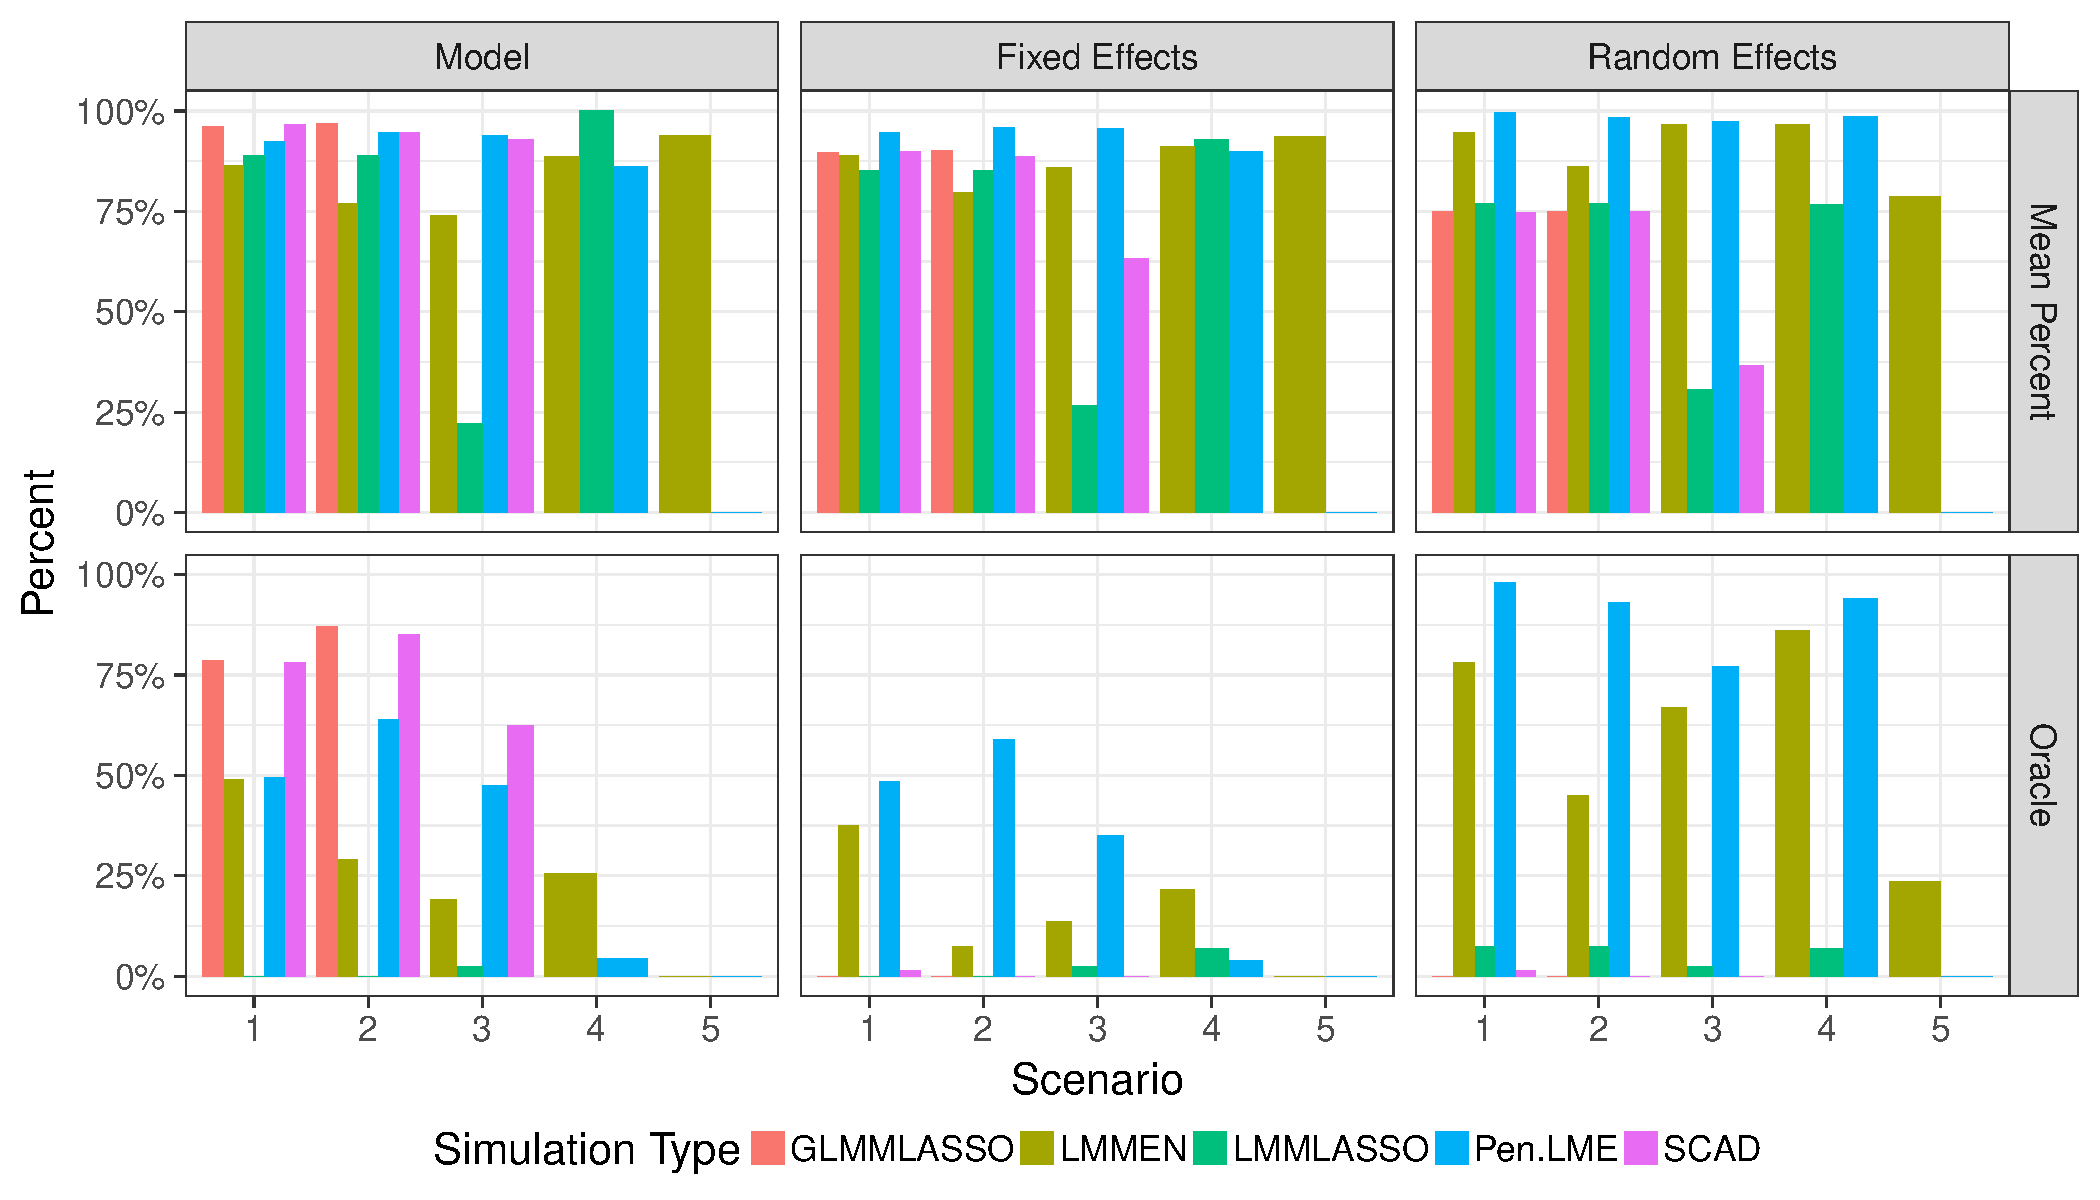
\includegraphics{figs/lmmen_paper-oracle}
\caption{Model selection performance comparison of Pen.LME (grey) and the LMMEN (black) for the simulations defined in Table \ref{tab:Scenario}. The panel columns from left to right are the selection performance by entire model, the fixed effects and the random effects. The panel rows depict the performance statistic, the upper row is the mean percent of parameters selected correctly, the bottom row measures the oracle property of each model.}
\label{fig:oracle}
\end{figure}
%
\section{Case Study}
The LMMEN algorithm was tested on high dimensional panel data accumulated as part the \href{http://www.goodjudgmentproject.com/}{Good Judgment Project} within the Aggregative Contingent Estimation (ACE) Program \footnote{Sponsored by the U.S. Intelligence Advanced Research Projects Activity (IARPA).}. The aim of this program is \textit{``to dramatically enhance the accuracy, precision, and timeliness of forecasts for a broad range of event types, through the development of advanced techniques that elicit, weight, and combine the judgments of many intelligence analysts."}. The study is characterized as a longitudinal study where probabilistic forecasts are derived from crowd sentiment.

The Good Judgment team recruited approximately 3,000 users in the first year. Those users were randomly assigned to 12 groups. There were 75 active questions  over the first year.  Each user could answer an active question at any time until the question was closed and resolved. This design is a natural one for a repeated measures model with random effects, in which the questions are designated as subjects with random intercepts and for each group a random effect is estimated. In addition there are 40 fixed variables that contain demographic, psychological and past performance information. The data tested was 100 random samples of 50 answers from 20 randomly sampled questions, giving a block structure of 1,000 observations.
%
    The LMMEN with specifications for the design structure will be compared to the Elastic Net algorithm, within the GLMNET R library\footnote{ \url{http://cran.r-project.org/web/packages/glmnet/index.html}. Version 2.0-2 was used in the simulations.} \cite{FHT2010}, which assumes an unstructured covariance design and crossvalidated levels of scaling parameters. The simple mean is used as the baseline aggregation method. Two levels of algorithm performance will be investigated, first is the model selection and second is the accuracy of the aggregated predictions. The statistic which will be used to test performance of the aggregated  predictions is the Brier score. In this case study only binary events are taken under consideration and 6 questions are omitted under this constraint. Thus the Brier score equation is defined as
\begin{equation*}
	BS=\frac{1}{N} \sum\limits_{t=1}^{N}(f_{t}-o)^2,
\end{equation*}
in which $f_t$ is the prediction at time $t$,  $o$ is the question outcome,  and $N$ is the number of prediction instances.
%
\begin{figure}[h]
\centering
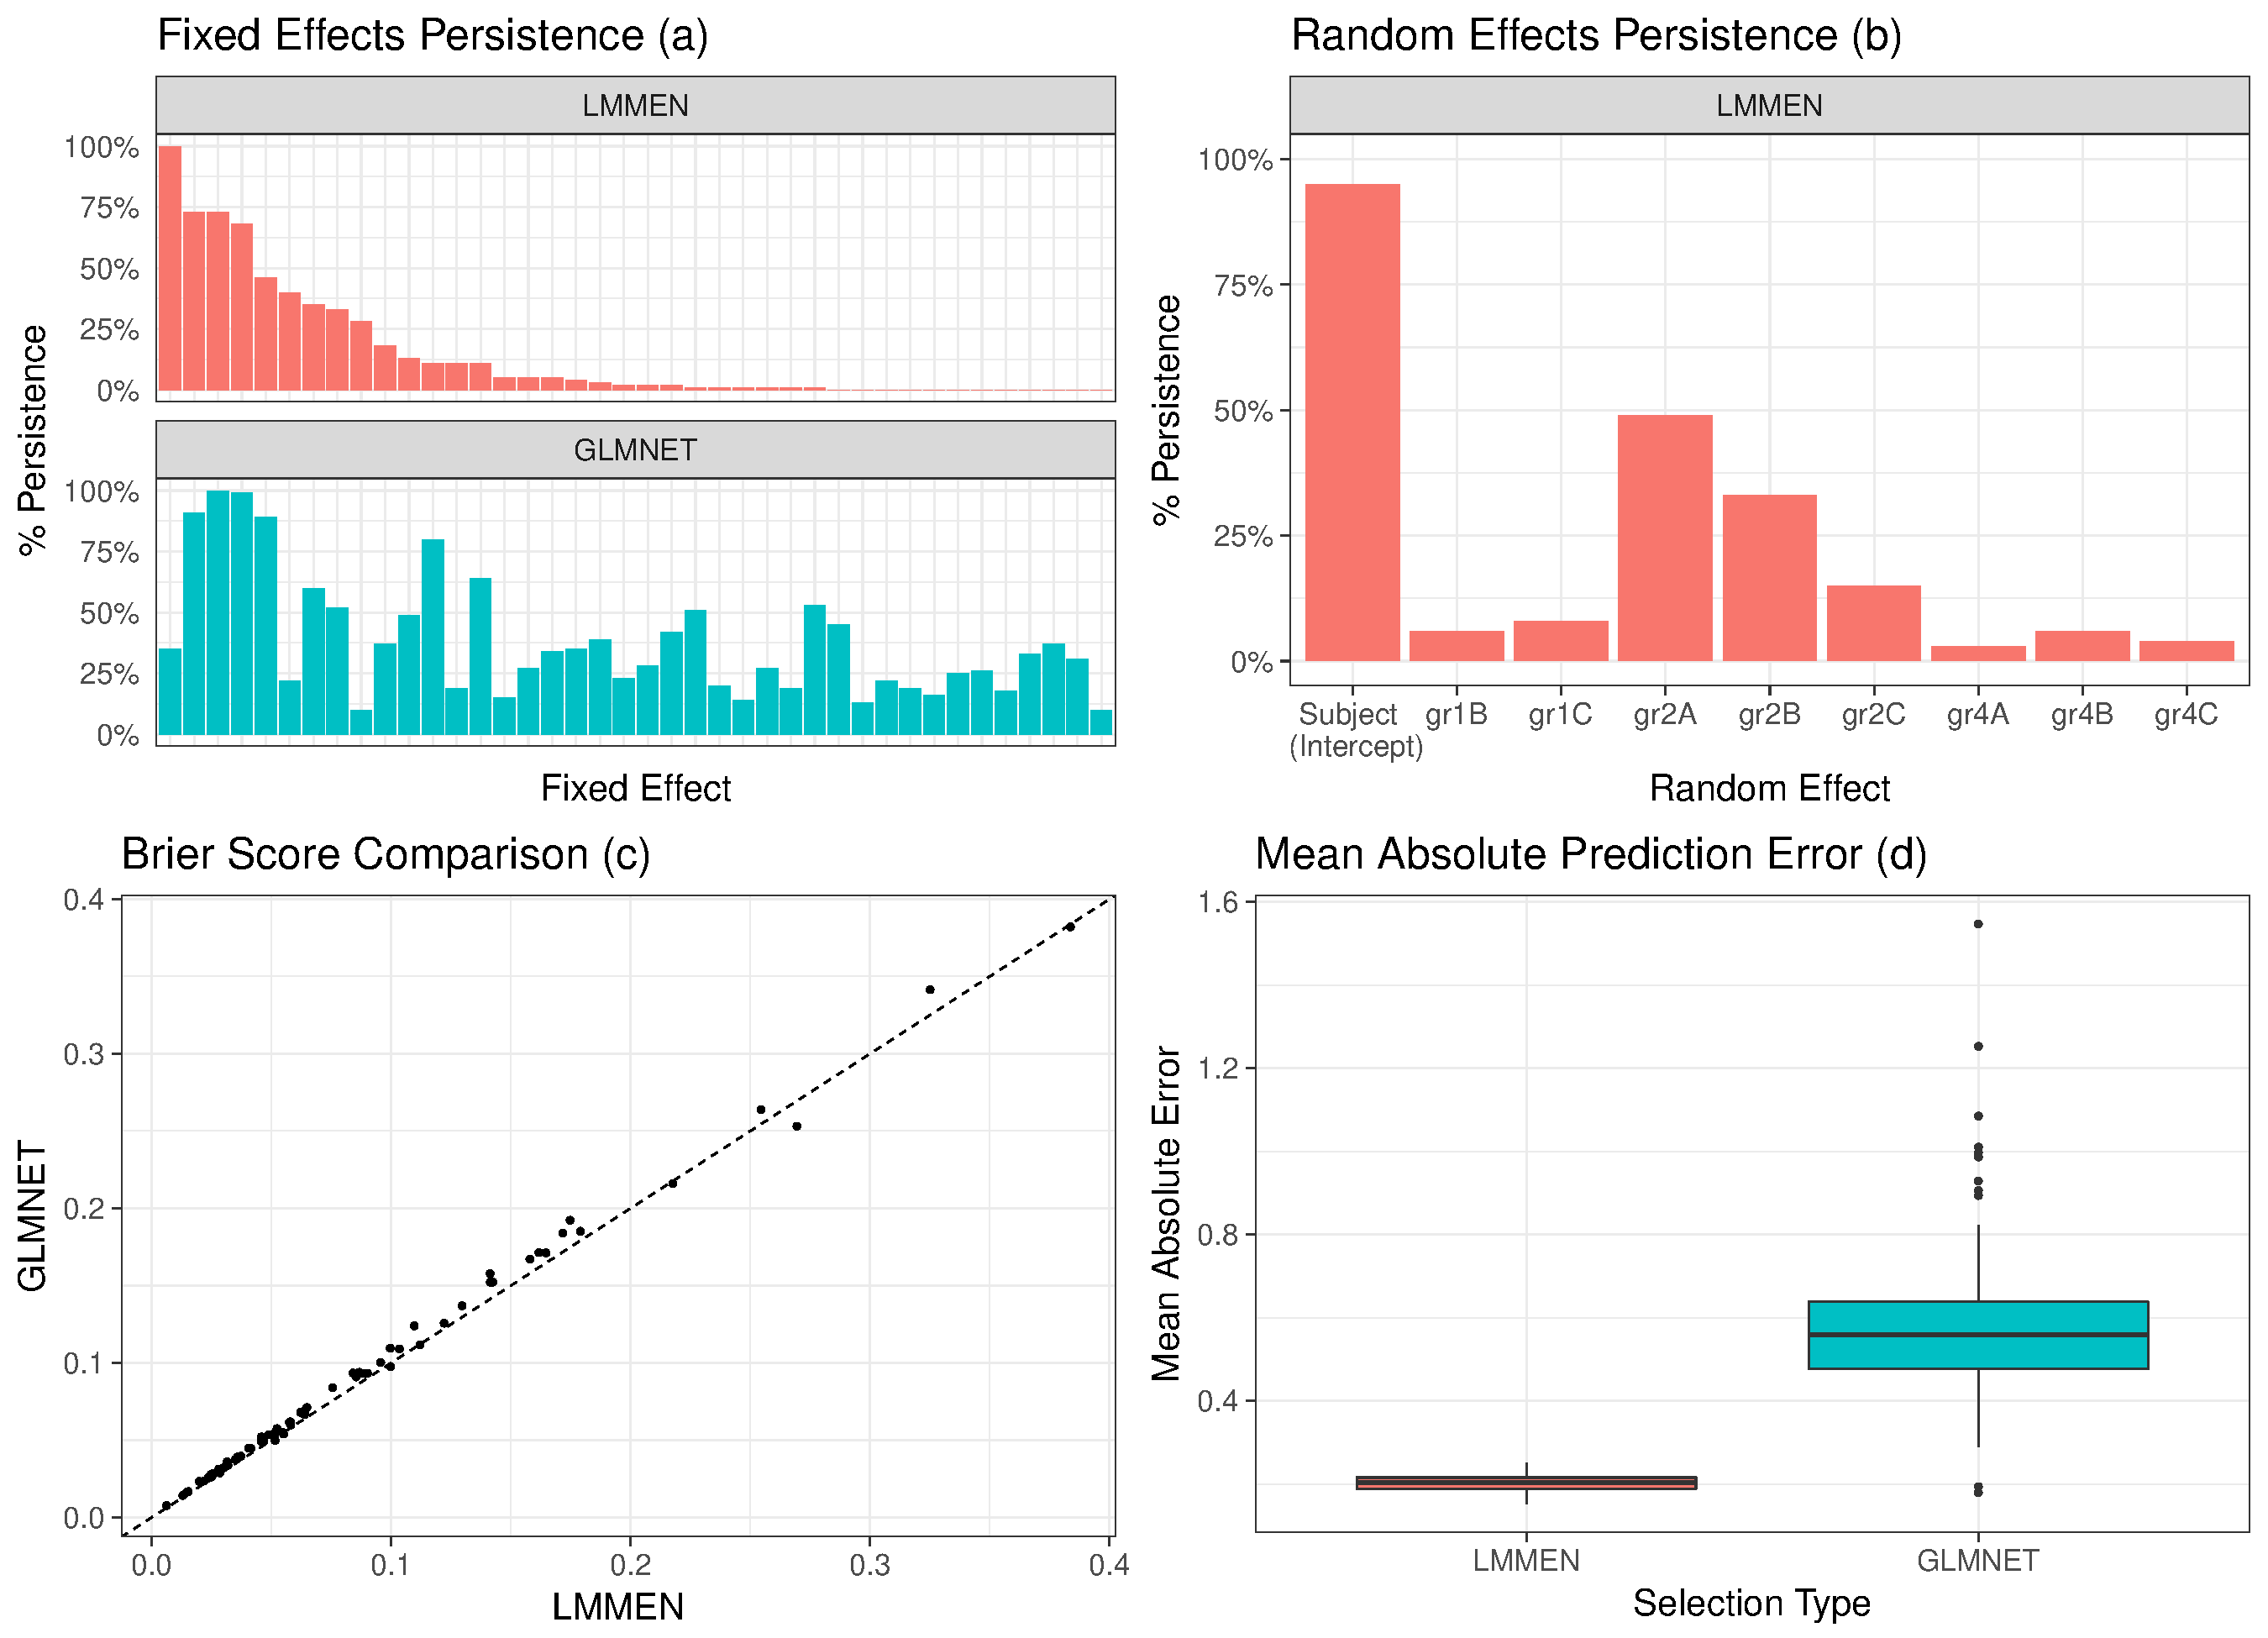
\includegraphics{figs/lmmen_paper-casepanel}
\caption{Model performance of GLMNET and LMMEN tested on 100 random samples of 1000 observations from the Good Judgment study. Panel (a) compares the distribution of fixed effects selection persistency between the two methods. Panel (b) depicts the random effects selection persistency of the LMMEN. Panel (c) compares the probabilistic forecast accuracy of the two methods using the Brier Score as the loss function. Panel (d) compares the distribution of the mean absolute prediction error of each method}
\label{fig:perform}
\end{figure}
%
First we compare the model selection between the two algorithms as seen in panel (a) of Figure \ref{fig:perform}. It can be seen that the LMMEN produces a higher level of sparsity than the GLMNET and the variables chosen are persistent in the simulation.
The addition of the design structure allows us to select random effects found in the data. The groups of users are assumed to be distributed normally with a variation parameter. After applying the LMMEN the optimal solution produces a sparse covariance matrix with relation to the random effects. The results of this selection can be found in panel (b) of Figure \ref{fig:perform}. We see that the variance estimate of groups \{1B,1C,4A,4B,4C\} is equal to zero in a large percent of the simulations, thus concluding that there is no difference between the user responses in those groups.

The second level of performance investigated is the prediction accuracy. The estimated non-zero covariates after selection are used to aggregate out of sample user predictions of active questions. The results of the two selection methods can be found in panel (c) of Figure \ref{fig:perform}. We see that both methods have low brier scores, i.e., the aggregated predictions are close to the final outcome. The average brier scores for GLMNET and LMMEN are .089 and .085 respectively. This shows that there is no major loss of prediction accuracy between the two selection methods. Both methods out perform the benchmark aggregation (grand mean) which has an average brier score of 0.11. The more significant difference as seen in panel (d) of Figure \ref{fig:perform} is the mean absolute prediction error, where in this case the average estimation error in the GLMNET is larger than the LMMEN. This reinforces the importance of modeling the structure of the data correctly in order to minimize errors in estimation.
\section{Discussion}
In the paper we have shown that fixed and random effects in high dimensional linear mixed models can be simultaneously selected. This selection method introduces the ability to select variables under conditions of multicollinearity both in the fixed and random effects. This method, LMMEN, furthers current variable selection of these models with the introduction of a ridge penalty into the optimization.

It was found through simulations that this method correctly selects fixed and random effects under sparse data designs. Simulations were carried out under the Gaussian assumption for both the conditional distribution and the distribution of the random effects. Further simulations will be carried out which relax the assumption of the conditional distribution. When testing the LMMEN in the case study the variable selection was comparable to a similar regularization method which does not model the covariance structure, GLMNET. The LMMEN gave further insight into the characteristics of groups of users, where a subset of them were found not have prediction difference within the groups.

This paper applies the Brier Score (L2 loss) as the loss function to tune the penalty parameters in the case study. One could calibrate the penalty parameters is the intraclass correlation (ICC) levels. The ICC is  intrinsic to random effects models, and is regularly used for evaluating the level of correlation between different groups as defined by the model. Applying the LMMEN while calibrating to minimize the ICC could be a vital tool for correctly selecting candidate random effects to model the data design and will be assessed in future work.
%\section{Appendix}
\appendix
\section{Appendix: proofs}
For the penalized log-likelihood in \eqref{eq:MLE-EN}, let $\phi=(\phi_1',0')'$ and let $$L^1(\phi_1)\equiv L\begin{Bmatrix}\begin{pmatrix}
\phi_1
\\ 0
\end{pmatrix}\end{Bmatrix} \text{ and } Q^1(\phi_1)\equiv Q
\begin{Bmatrix}
\begin{pmatrix}
\phi_1
\\ 0
\end{pmatrix}
\end{Bmatrix}$$ denote the log-likelihood and the penalized log-likelihood of the first $s$ components of $\phi$.


\begin{proof}[Proof Theorem 1]
	Consider the penalized log-likelihood $Q(\phi)$ given in \eqref{eq:MLE-EN} in the neighborhood of the true value $ \phi_{10} $. Let $u\ne 0$, and $\phi_1=\phi_{10}+w_mu$. Setting $\phi_2=0$, we show that for a small enough $\epsilon>0$, there exists a large constant $C$ such that for a sufficiently large $m$,
	\begin{equation*}
	P\Bigl(  \sup_{\|u\|=C}Q^1(
	\phi_{10}+w_mu)  <
	Q(\phi_{10})
	\Bigr) \ge 1-\epsilon.
	\end{equation*}
Thus, with probability $1-\epsilon$ the maximum is within the ball of radios $Cw_m$.

Note that\begin{align*}
mD_m(u)&\equiv    Q^1(\phi_1)-Q^1(\phi_{10})
\\
&=-\left[ L^1(\phi_{10}+w_mu)-L^1(\phi_{10})\right]
\\
&\hspace{2em} +\lambda_1^f\bigl(\|\beta_0+w_m u_\beta\|_1-\|\beta_0\|_1\bigr) +\lambda_1^r\bigl(\|d_0+w_m u_d\|_1-\|d_0\|_1\bigr)
\\
&\hspace{2em} +\lambda_2^f\bigl(\|\beta_0+w_m u_\beta\|_2^2-\|\beta_0\|_2^2\bigr) +\lambda_2^r\bigl(\|d_0+w_m u_d\|_2^2-\|d_0\|_2^2\bigr),
\end{align*}
where we divided $u$ to its  natural components $u_\beta\in R^p$ and $u_d\in R^q$.  Using the Taylor series expansion we have
\begin{align*}
&D_m(u)
\\
&=-w_m(m^{-1}\nabla L(\phi_{10}))'u -\frac{w_m^2}{2m}u'[\nabla^2L(\phi_{10})]u +R_m
\\
&\hspace{2em} +m^{-1}\lambda_1^f\bigl(\|\beta_0+w_m u_\beta\|_1-\|\beta_0\|_1\bigr) +m^{-1}\lambda_1^r\bigl(\|d_0+w_m u_d\|_1-\|d_0\|_1\bigr)
\\
&\hspace{2em} +m^{-1}\lambda_2^f\bigl(\|\beta_0+w_m u_\beta\|_2^2-\|\beta_0\|_2^2\bigr) +m^{-1}\lambda_2^r\bigl(\|d_0+w_m u_d\|_2^2-\|d_0\|_2^2\bigr),
\end{align*}
%
where $\nabla L(\phi_{10}),\nabla^2 L(\phi_{10})$ denote the vector and matrix of the first and second order partial derivatives of $L(\phi_{1})$  at $\phi_{10}$ respectively. $\nabla P(\beta,d),\nabla^2P(\beta,d)$ denote the first and second derivatives of the penalty term at $(\beta_0,d_0)$. The remainder $R_n$  tends to zero as m $\rightarrow \infty$ since, by \nameref{C2}, $|R_m|$ can be bounded by
$$\left( \frac{w_m^3\|u\|_2^3}{6m}\right) \sum\limits_{i=1}^{m} M(y_i,X_i,Z_i) = O_P( w_m^{3}).$$


The $j${th} partial derivative for each corresponding $\beta_1,d_1,\gamma_1$  the $\nabla L(\phi_{10})$ satisfies
$E\left\lbrace \frac{\partial}{\partial \beta_j}L(\phi_1)\right\rbrace=E\left\lbrace \frac{\partial}{\partial d_j}L(\phi_1)\right\rbrace=E\left\lbrace \frac{\partial}{\partial \gamma_j}L(\phi_1)\right\rbrace=0$ and thus the corresponding empirical means  are $O_p(m^{-1/2})$.

For $\nabla^2 L(\phi_{10})$ we have $$m^{-1} \nabla^2 L(\phi_{10}) \rightarrow_p -I(\phi_{10}),$$ where $I(\phi_{10})$ is the Fisher information evaluated at $\phi_{10}$, which is  positive definite by  (\nameref{C1}). By choosing a sufficiently large $C$, the second term dominates the first term uniformly in $\|u\|=C$.

For the penalty term if $w_mP(\beta,d) \rightarrow 0$ as $m \rightarrow \infty$ it follows that $P(\beta,d) \rightarrow_p 0$, and thus also dominated by the second term.  The absolute value of the  penalty component of $D_m(u)$ is bounded by
\begin{align*}
&\hspace{-2em} m^{-1}w_m\lambda_1^f\|u_\beta\|_1 +m^{-1}w_m\lambda_1^r\|u_d\|_1
  +m^{-1}\lambda_2^f\bigl(2w_m\|\beta_0\|_2 \|u_\beta\|_2 +w_m^2\|u_0\|_2^2\bigr)
\\
&\hspace{2em} +m^{-1}\lambda_2^r\bigl(2w_m\|d_0\|_2 \|u_d\|_2+w_m^2\|u_d\|_2^2\bigr)
\\
&\le m^{-1}w_mC\bigl(\lambda_1^f\sqrt s  +\lambda_1^r\sqrt s   +\lambda_2^f(2\|\beta_0\|_2  + w_m C)  +\lambda_2^r(2\|d_0\|_2  + w_m C)\bigr).
\end{align*}
%$$w_m^2 C^2> \frac{w_m C\lambda_1 \sqrt s}{m} + \frac{\lambda_2 w_m^2 c^2}{m} + \frac{\lambda_2 w_m C p }{m}  $$
%$$ 1> \frac{\lambda_1 \sqrt s}{m w_m C} + \frac{\lambda_2 }{m} + \frac{\lambda_2  s }{m w_m C}  $$
which is dominated by the second term of $D_m(u)$. Therefore, by choosing  a sufficiently large $C$ there exists a local maximum inside $\left\lbrace\phi_{10}+w_mu:\|u\|<C \right\rbrace$  with probability $1-\epsilon$, thus there exists a local maximizer $\hat{\phi}=(\hat{\phi_1}',0')'$ of $\phi_0=(\phi_1',0')'$ such that $\|\hat{\phi_1}-\phi_{10}\|=O_p(w_m)$.
\end{proof}
For the following proof we define $\phi=(\beta',d',\gamma')$ as a $k \times 1$ vector of unknown parameters of size $k=k_{\beta}+k_d+k_{\gamma}$. Let $\phi_2=(\beta'_2,d'_2,\gamma'_2)$ be a vector of size $k_2=k-s$ corresponding to the true zero parameters, given $k_2=k_{\beta_2}+k_{d_2}+k_{\gamma_2}$. Reminding that we defined earlier that the likelihood and the penalized log likelihood as
$$L(\phi)=L\begin{Bmatrix}
\begin{pmatrix}
\phi_1 \\ \phi_2
\end{pmatrix}
\end{Bmatrix} \text{ and } Q(\phi)=Q\begin{Bmatrix}
\begin{pmatrix}
\phi_1 \\ \phi_2
\end{pmatrix}
\end{Bmatrix}.$$
\begin{proof}[Proof Theorem 2]
For $m\rightarrow\infty$ and any $\phi_1:||\phi_1-\phi_{10}||_1\le Mm^{-1/2}$ and for  $\epsilon_m=Mm^{-1/2}$ and for each $j=(s+1),\dots,(k_{\beta_2}+k_{d_2})$ we have with probability tending to 1 that
\begin{align}
\label{eq:derivQ}
\frac{\partial}{\partial\varphi_j}Q(\phi)<0 \text{ for } & 0<\varphi_j<\epsilon_m
\\
\frac{\partial}{\partial\varphi_j}Q(\phi)>0 \text{ for } & -\epsilon_m<\varphi_j<0 \nonumber
\end{align}
The partial derivative of $Q(\phi)$ with respect to $\varphi_j$ is given by:
$$\frac{\partial}{\partial\varphi_j}Q(\phi)
=\frac{\partial}{\partial\varphi_j}L(\phi)-\left( \lambda_1\text{sgn}(\varphi_j)+2\lambda_2\varphi_j\right),$$ noting that the penalty is dependent on whether $\varphi_j$ is $\beta$ or d.

One can verify \eqref{eq:derivQ} through the Taylor Series expansion  of $\frac{\partial}{\partial\varphi_j}L(\phi)=\frac{\partial}{\partial\varphi_j}L(\phi)$ around $\phi_0$:
\begin{align}
\label{eq:derivQTaylor}
\frac{\partial}{\partial\varphi_j} Q(\phi) =&\frac{\partial}{\partial\varphi_j}L(\phi_0) -\sum_{l=1}^{k}\frac{\partial}{\partial\varphi_l} \left(\frac{\partial}{\partial\varphi_j}L(\phi_0)\right) (\varphi_l-\varphi_{l0})
\\
+&\frac{1}{2} \sum_{i=1}^{m} \sum_{l=1}^{k} \sum_{g=1}^{k} \frac{\partial^2}{\partial\varphi_l\partial\varphi_g} \left(\frac{\partial}{\partial\varphi_j}L_i(\phi_*)\right) (\varphi_l-\varphi_{l0}) (\varphi_g-\varphi_{g0}) \nonumber
\\
-&\left( \lambda_1\text{sgn}(\varphi_j)+2\lambda_2\varphi_j\right), \nonumber
\end{align}
where $\phi_*$ is on the interval connecting $\phi$ and $\phi_0$. Next we define the first order derivatives needed to numerically solve \eqref{eq:derivQTaylor}:
\begin{align*}
L_{\beta}=&\frac{\partial}{\partial\beta_j}L(\phi_0)=X'_jV^{-1}(y-X\beta)=O_p(m^{-1/2})\\
L_{d}=&\frac{\partial}{\partial d_j}L(\phi_0)=\frac{1}{2}\left[ \Tr(V^{-1}S^j)+(y-X\beta)'(V^{-1}S^jV^{-1})(y-X\beta)\right]=O_p(m^{-1/2}),
\end{align*}
where $S^j=Z(\frac{\partial}{\partial d_j}D\Gamma\Gamma'D)Z'$ and $\Tr(A)$ is the trace operator on a given matrix A. We now define the second order derivatives which follow $\frac{1}{m}\nabla^2L(\phi)|_{\phi=\phi_0}\rightarrow E_{\phi_1=\phi_{10}}[\nabla^2L(\phi)]$, where
\begin{equation*}
E[\nabla^2L(\phi)]=E
\left[ \begin{array}{ccc}
L_{\beta\beta}&L_{\beta d}&L_{\beta\gamma}\\
L'_{\beta d}&L_{dd}&L_{d\gamma}\\
L'_{\beta\gamma}&L'_{d\gamma}&L_{\gamma\gamma}
\end{array}\right],
\end{equation*}
\begin{align*}
E[L_{\beta\beta}]_j=&-XV^{-1}X\\
E[L_{\beta d}]_j=&-E\left[X'_j(V^{-1}S^jV^{-1})(y-X\beta)\right]|_{\phi=\phi_0}=0\\
E[L_{\beta\gamma}]_j=&-E\left[X'_j(V^{-1}T^jV^{-1})(y-X\beta)\right]|_{\phi=\phi_0}=0 \nonumber\\
E[L_{dd}]_{jl}=&-\Tr(V^{-1}S^jV^{-1}S^l)|_{\left\lbrace j\ge (s+1),\phi_j=0\right\rbrace }=0\\
E[L_{\gamma\gamma}]_{jl}=&-\Tr(V^{-1}T^jV^{-1}T^l)|_{\left\lbrace j\ge (s+1),\phi_j=0\right\rbrace }=0 \nonumber\\
E[L_{d\gamma}]_{jl}=&-\Tr(V^{-1}S^jV^{-1}T^l)|_{\left\lbrace j\ge (s+1),\phi_j=0\right\rbrace }=0 \nonumber,
\end{align*}
where $T^j=ZD(\frac{\partial}{\partial \gamma_j}\Gamma\Gamma')DZ'$.\\ Using these partial derivatives we solve \eqref{eq:derivQTaylor} first for $\phi_j=\beta_j$ and then for $\phi_j=d_j$.
\begin{align*}
 &\frac{1}{\sqrt{m}}\left(\frac{\partial}{\partial \beta_j}Q(\phi)\right)
 \\=
 &\frac{1}{\sqrt{m}} \Biggl [ L_{\beta}
 -m\left(\sum_{l=1}^{k_{\beta}}L_{\beta\beta}(\beta_l-\beta_{l0})
 +\sum_{l=k_{\beta+1}}^{k_{d}}L_{\beta d}(d_l-d_{l0})
 +\sum_{l=k_{d+1}}^{k_{\gamma}}L_{\beta\gamma}(\gamma_l-\gamma_{l0})\right)	\\&
 +\sum_{i=1}^{m}\sum_{l=1}^{k_{\beta}}\sum_{g=k_{\beta}+1}^{k_d}\frac{\partial}{\partial \beta_g}L_{\beta d}(\beta_l-\beta_{l0})(d_g-d_{g0})
 \\&
 +\sum_{i=1}^{m}\sum_{l=1}^{k_{\beta}}\sum_{g=k_{d}+1}^{k_{\gamma}}\frac{\partial}{\partial \beta_g}L_{\beta \gamma}(\beta_l-\beta_{l0})(\gamma_g-\gamma_{g0})
 \\
 &+\sum_{i=1}^{m}\sum_{l=k_{\beta}+1}^{k_d}\sum_{g=k_{d+1}}^{k_{\gamma}}\frac{\partial}{\partial \gamma_g}L_{\beta d}(d_l-d_{l0})(\gamma_g-\gamma_{g0})
 \\
 &+\frac{1}{2}\Biggr(\sum_{i=1}^{m}\sum_{l=k_{\beta}+1}^{k_d}\sum_{g=k_{\beta}+1}^{k_d}\frac{\partial}{\partial d_g}L_{\beta d}(d_l-d_{l0})(d_g-d_{g0})
 \\
 &+\sum_{i=1}^{m}\sum_{l=k_d+1}^{k_{\gamma}}\sum_{g=k_{d+1}}^{k_{\gamma}}\frac{\partial}{\partial \gamma_g}L_{\beta \gamma}(\gamma_l-\gamma_{l0})(\gamma_g-\gamma_{g0})\Biggr)
 -\left(\lambda^f_1\text{sgn}(\beta_j)+2\lambda_2^f(\beta_j)\right)
  \Biggr],
\end{align*}
given $||\phi-\phi_0||_1\le Mm^{-1/2}$ then we have {\footnotesize
\begin{equation}
\frac{1}{\sqrt{m}}\left(\frac{\partial}{\partial \beta_j}Q(\phi)\right)=-\left(\lambda^f_1\text{sgn}(\beta_j)+2\lambda_2^f(\beta_j)\right)+O_p(1).
\end{equation}}
For $\beta_{j0}=0$ and $\lbrace\lambda^f_1,\lambda^f_2\rbrace\rightarrow \infty$ the sign of the derivative is completely determined by $\beta_j$, more specifically:
\begin{equation*}
\begin{array}{cccc}
\text{if} & M>\beta_j>0&\text{then}&\frac{\partial}{\partial \beta_j}Q(\phi)<0
\\
\text{if} & -M<\beta_j<0&\text{then}&\frac{\partial}{\partial \beta_j}Q(\phi)>0
\end{array}.
\end{equation*}
Similarly,
\begin{align}\notag
 &\frac{1}{\sqrt{m}}\left(\frac{\partial}{\partial d_j}Q(\phi)\right)
 \\\notag
 &=\frac{1}{\sqrt{m}} \Biggl [ L_{d}
 -m\left(\sum_{l=1}^{k_{\beta}}L_{\beta\beta}(\beta_l-\beta_{l0})
 +\sum_{l=k_{\beta+1}}^{k_{d}}L_{\beta d}(d_l-d_{l0})
 +\sum_{l=k_{d+1}}^{k_{\gamma}}L_{\beta\gamma}(\gamma_l-\gamma_{l0})\right)
 \\\notag\displaybreak	&\hspace{2em}+\sum_{i=1}^{m}\sum_{l=1}^{k_{\beta}}\sum_{g=1}^{k_{\beta}}\frac{\partial}{\partial \beta_g}L_{d\beta}(\beta_l-\beta_{l0})(\beta_g-\beta_{g0})
 \\\notag
 &\hspace{2em}+\sum_{i=1}^{m}\sum_{l=k_{\beta}+1}^{k_d}\sum_{g=k_{d}+1}^{k_{\gamma}}\frac{\partial}{\partial \gamma_g}L_{d d}(d_l-d_{l0})(\gamma_g-\gamma_{g0})
 \\\notag
 &\hspace{2em}+\sum_{i=1}^{m}\sum_{l=k_{\beta}+1}^{k_d}\sum_{g=k_{d+1}}^{k_{\gamma}}\frac{\partial}{\partial d_g}L_{ d\beta}(\beta_l-\beta_{l0})(d_g-d_{g0})
 \\\notag
 &\hspace{2em}+\frac{1}{2}\Biggr(\sum_{i=1}^{m}\sum_{l=k_{\beta}+1}^{k_d}\sum_{g=k_{\beta}+1}^{k_d}\frac{\partial}{\partial d_g}L_{d d}(d_l-d_{l0})(d_g-d_{g0})
 \\\notag
 &\hspace{2em}+\sum_{i=1}^{m}\sum_{l=k_d+1}^{k_{\gamma}}\sum_{g=k_{d+1}}^{k_{\gamma}}\frac{\partial}{\partial \gamma_g}L_{d \gamma}(\gamma_l-\gamma_{l0})(\gamma_g-\gamma_{g0})\Biggr)-\left(\lambda^r_1\text{sgn}(d_j)+2\lambda_2^r(d_j)\right)
  \Biggr],
\end{align}
given $||\phi-\phi_0||_1\le Mm^{-1/2}$ then we have {\footnotesize
\begin{equation*}
\frac{1}{\sqrt{m}}\left(\frac{\partial}{\partial d_j}Q(\phi)\right)=-\left(\lambda^r_1\text{sgn}(d_j)+2\lambda_2^r(d_j)\right)+O_p(1).
\end{equation*}}
For $d_{j0}=0$ and $(\lambda^r_1,\lambda^r_2)\rightarrow \infty$ the sign of the derivative is completely determined by $d_j$, more specifically:
{
	\begin{equation*}
	\begin{array}{cccc}
	\text{if} & M>d_j>0&\text{then}&\frac{\partial}{\partial d_j}Q(\phi)<0
\\
	\text{if} & -M<d_j<0&\text{then}&\frac{\partial}{\partial d_j}Q(\phi)>0
\\
	\end{array}.
	\end{equation*}}
\end{proof} 
\bibliography{lmmen_bib}{}
\end{document}
